\begin{quote}
This is part 25 of Categories for Programmers. Previously:
\href{https://bartoszmilewski.com/2017/02/28/f-algebras/}{F-Algebras}.
See the
\href{https://bartoszmilewski.com/2014/10/28/category-theory-for-programmers-the-preface/}{Table
of Contents}.
\end{quote}

If we interpret endofunctors as ways of defining expressions, algebras
let us evaluate them and monads let us form and manipulate them. By
combining algebras with monads we not only gain a lot of functionality
but we can also answer a few interesting questions. One such question
concerns the relation between monads and adjunctions. As we've seen,
every adjunction
\href{https://bartoszmilewski.com/2016/12/27/monads-categorically/}{defines
a monad} (and a comonad). The question is: Can every monad (comonad) be
derived from an adjunction? The answer is positive. There is a whole
family of adjunctions that generate a given monad. I'll show you two
such adjunction.\\
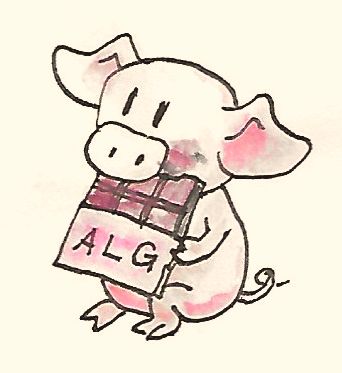
\includegraphics[width=1.27083in]{images/pigalg.png}\\
Let's review the definitions. A monad is an endofunctor \code{m}
equipped with two natural transformations that satisfy some coherence
conditions. The components of these transformations at \code{a} are:

\begin{verbatim}
ηa :: a -> m a μa :: m (m a) -> m a
\end{verbatim}

An algebra for the same endofunctor is a selection of a particular
object --- the carrier \code{a} --- together with the morphism:

\begin{verbatim}
alg :: m a -> a
\end{verbatim}

The first thing to notice is that the algebra goes in the opposite
direction to \code{ηa}. The intuition is that \code{ηa} creates a
trivial expression from a value of type \code{a}. The first coherence
condition that makes the algebra compatible with the monad ensures that
evaluating this expression using the algebra whose carrier is \code{a}
gives us back the original value:

\begin{verbatim}
alg ∘ ηa = ida
\end{verbatim}

The second condition arises from the fact that there are two ways of
evaluating the doubly nested expression \code{m\ (m\ a)}. We can first
apply \code{μa} to flatten the expression, and then use the evaluator
of the algebra; or we can apply the lifted evaluator to evaluate the
inner expressions, and then apply the evaluator to the result. We'd like
the two strategies to be equivalent:

\begin{verbatim}
alg ∘ μa = alg ∘ m alg
\end{verbatim}

Here, \code{m\ alg} is the morphism resulting from lifting
\code{alg} using the functor \code{m}. The following commuting
diagrams describe the two conditions (I replaced \code{m} with
\code{T} in anticipation of what follows):

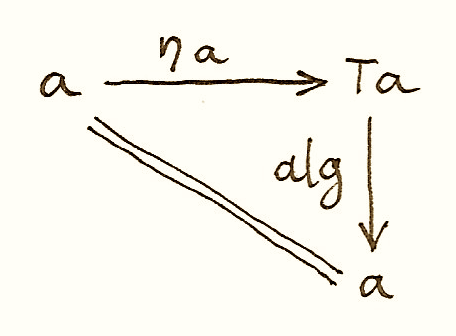
\includegraphics[width=1.81250in]{images/talg1.png}

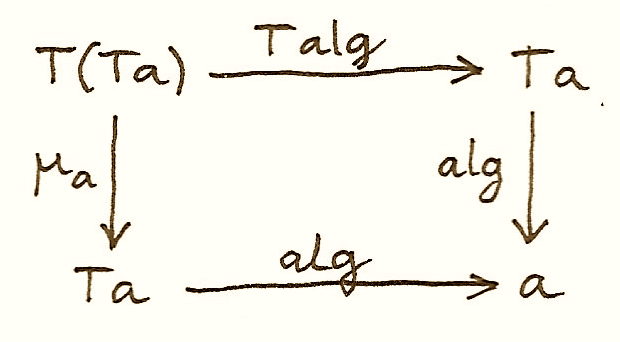
\includegraphics[width=2.40625in]{images/talg2.png}

We can also express these condition in Haskell:

\begin{verbatim}
alg . return = id alg . join = alg . fmap alg
\end{verbatim}

Let's look at a small example. An algebra for a list endofunctor
consists of some type \code{a} and a function that produces an
\code{a} from a list of \code{a}. We can express this function using
\code{foldr} by choosing both the element type and the accumulator
type to be equal to \code{a}:

\begin{verbatim}
foldr :: (a -> a -> a) -> a -> [a] -> a
\end{verbatim}

This particular algebra is specified by a two-argument function, let's
call it \code{f}, and a value \code{z}. The list functor happens to
also be a monad, with \code{return} turning a value into a singleton
list. The composition of the algebra, here \code{foldr\ f\ z}, after
\code{return} takes \code{x} to:

\begin{verbatim}
foldr f z [x] = x `f` z
\end{verbatim}

where the action of \code{f} is written in the infix notation. The
algebra is compatible with the monad if the following coherence
condition is satisfied for every \code{x}:

\begin{verbatim}
x `f` z = x
\end{verbatim}

If we look at \code{f} as a binary operator, this condition tells us
that \code{z} is the right unit.

The second coherence condition operates on a list of lists. The action
of \code{join} concatenates the individual lists. We can then fold the
resulting list. On the other hand, we can first fold the individual
lists, and then fold the resulting list. Again, if we interpret
\code{f} as a binary operator, this condition tells us that this
binary operation is associative. These conditions are certainly
fulfilled when \code{(a,\ f,\ z)} is a monoid.

\subsection{T-algebras}\label{t-algebras}

Since mathematicians prefer to call their monads \code{T}, they call
algebras compatible with them T-algebras. T-algebras for a given monad T
in a category \emph{C} form a category called the Eilenberg-Moore
category, often denoted by C\textsuperscript{T}. Morphisms in that
category are homomorphisms of algebras. These are the same homomorphisms
we've seen defined for F-algebras.

A T-algebra is a pair consisting of a carrier object and an evaluator,
\code{(a,\ f)}. There is an obvious forgetful functor \code{UT} from
C\textsuperscript{T} to C, which maps \code{(a,\ f)} to \code{a}. It
also maps a homomorphism of T-algebras to a corresponding morphism
between carrier objects in C. You may remember from our discussion of
adjunctions that the left adjoint to a forgetful functor is called a
free functor.

The left adjoint to \code{UT} is called \code{FT}. It maps an object
\code{a} in C to a free algebra in C\textsuperscript{T}. The carrier
of this free algebra is \code{T\ a}. Its evaluator is a morphism from
\code{T\ (T\ a)} back to \code{T\ a}. Since \code{T} is a monad,
we can use the monadic \code{μa} (Haskell \code{join}) as the
evaluator.

We still have to show that this is a T-algebra. For that, two coherence
conditions must be satisified:

\begin{verbatim}
alg ∘ ηTa = idTa
\end{verbatim}

\begin{verbatim}
alg ∘ μa = alg ∘ T alg
\end{verbatim}

But these are just monadic laws, if you plug in \code{μ} for the
algebra.

As you may recall, every adjunction defines a monad. It turns out that
the adjunction between F\textsuperscript{T} and U\textsuperscript{T}
defines the very monad \code{T} that was used in the construction of
the Eilenberg-Moore category. Since we can perform this construction for
every monad, we conclude that every monad can be generated from an
adjunction. Later I'll show you that there is another adjunction that
generates the same monad.

Here's the plan: First I'll show you that \code{FT} is indeed the left
adjoint of \code{UT}. I'll do it by defining the unit and the counit
of this adjunction and proving that the corresponding triangular
identities are satisfied. Then I'll show you that the monad generated by
this adjunction is indeed our original monad.

The unit of the adjunction is the natural transformation:

\begin{verbatim}
η :: I -> UT ∘ FT
\end{verbatim}

Let's calculate the \code{a} component of this transformation. The
identity functor gives us \code{a}. The free functor produces the free
algebra \code{(T\ a,\ μa)}, and the forgetful functor reduces it to
\code{T\ a}. Altogether we get a mapping from \code{a} to
\code{T\ a}. We'll simply use the unit of the monad \code{T} as the
unit of this adjunction.

Let's look at the counit:

\begin{verbatim}
ε :: FT ∘ UT -> I
\end{verbatim}

Let's calculate its component at some T-algebra \code{(a,\ f)}. The
forgetful functor forgets the \code{f}, and the free functor produces
the pair \code{(T\ a,\ μa)}. So in order to define the component of
the counit \code{ε} at \code{(a,\ f)}, we need the right morphism in
the Eilenberg-Moore category, or a homomorphism of T-algebras:

\begin{verbatim}
(T a, μa) -> (a, f)
\end{verbatim}

Such homomorphism should map the carrier \code{T\ a} to \code{a}.
Let's just resurrect the forgotten evaluator \code{f}. This time we'll
use it as a homomorphism of T-algebras. Indeed, the same commuting
diagram that makes \code{f} a T-algebra may be re-interpreted to show
that it's a homomorphism of T-algebras:

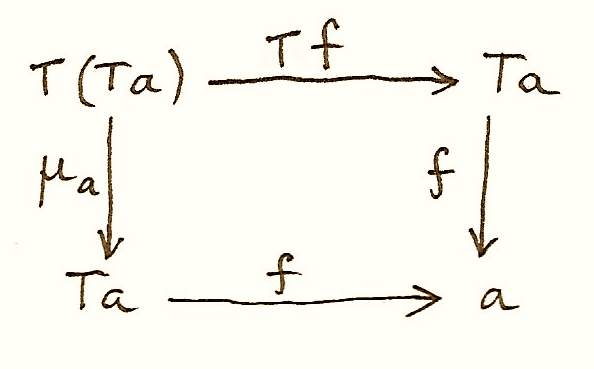
\includegraphics[width=2.57292in]{images/talg31.png}\\
We have thus defined the component of the counit natural transformation
\code{ε} at \code{(a,\ f)} (an object in the category of T-algebras)
to be \code{f}.

To complete the adjunction we also need to show that the unit and the
counit satisfy triangular identites. These are:

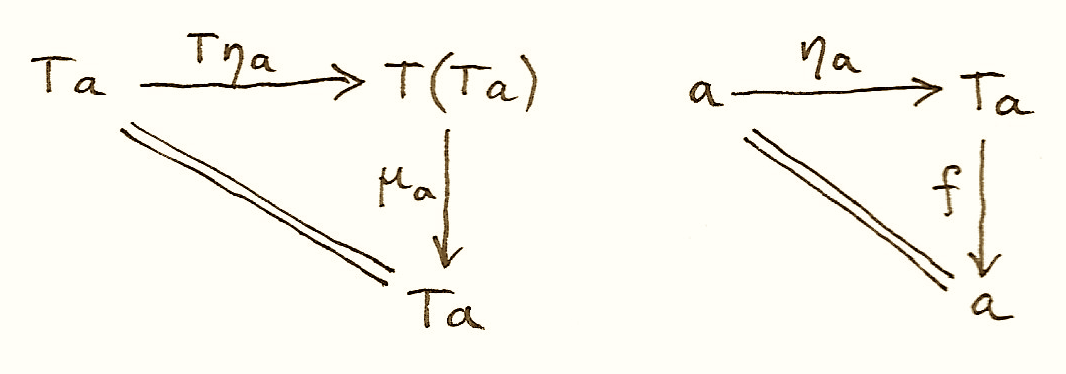
\includegraphics[width=4.64583in]{images/talg4.png}

The first one holds because of the unit law for the monad \code{T}.
The second is just the law of the T-algebra \code{(a,\ f)}.

We have established that the two functors form an adjunction:

\begin{verbatim}
FT ⊣ UT
\end{verbatim}

Every adjunction gives rise to a monad. The round trip

\begin{verbatim}
UT ∘ FT
\end{verbatim}

is the endofunctor in C that gives rise to the corresponding monad.
Let's see what its action on an object \code{a} is. The free algebra
created by \code{FT} is \code{(T\ a,\ μa)}. The forgetful functor
\code{FT} drops the evaluator. So, indeed, we have:

\begin{verbatim}
UT ∘ FT = T
\end{verbatim}

As expected, the unit of the adjunction is the unit of the monad
\code{T}.

You may remember that the counint of the adjunction produces monadic
muliplication through the following formula:

\begin{verbatim}
μ = R ∘ ε ∘ L
\end{verbatim}

This is a horizontal composition of three natural transformations, two
of them being identity natural transformations mapping, respectively,
\code{L} to \code{L} and \code{R} to \code{R}. The one in the
middle, the counit, is a natural transformation whose component at an
algebra \code{(a,\ f)} is \code{f}.

Let's calculate the component \code{μa}. We first horizontally compose
\code{ε} after \code{FT}, which results in the component of
\code{ε} at \code{FTa}. Since \code{FT} takes \code{a} to the
algebra \code{(T\ a,\ μa)}, and \code{ε} picks the evaluator, we end
up with \code{μa}. Horizontal composition on the left with \code{UT}
doesn't change anything, since the action of \code{UT} on morphisms is
trivial. So, indeed, the \code{μ} obtained from the adjunction is the
same as the \code{μ} of the original monad \code{T}.

\subsection{The Kleisli Category}\label{the-kleisli-category}

We've seen the Kleisli category before. It's a category constructed from
another category \emph{C} and a monad \code{T}. We'll call this
category \emph{C\textsubscript{T}}. The objects in the Kleisli category
\emph{C\textsubscript{T}} are the objects of \emph{C}, but the morphisms
are different. A morphism \code{fK} from \code{a} to \code{b} in
the Kleisli category corresponds to a morphism \code{f} from
\code{a} to \code{T\ b} in the original category. We call this
morphism a Kleisli arrow from \code{a} to \code{b}.

Composition of morphisms in the Kleisli category is defined in terms of
monadic composition of Kleisli arrows. For instance, let's compose
\code{gK} after \code{fK}. In the Kleisli category we have:

\begin{verbatim}
fK :: a -> b gK :: b -> c
\end{verbatim}

which, in the category \emph{C}, corresponds to:

\begin{verbatim}
f :: a -> T b g :: b -> T c
\end{verbatim}

We define the composition:

\begin{verbatim}
hK = gK ∘ fK
\end{verbatim}

as a Kleisli arrow in \emph{C}

\begin{verbatim}
h :: a -> T c h = μ ∘ (T g) ∘ f
\end{verbatim}

In Haskell we would write it as:

\begin{verbatim}
h = join . fmap g . f
\end{verbatim}

There is a functor \code{F} from \emph{C} to \emph{C\textsubscript{T}}
which acts trivially on objects. On morphims, it maps \code{f} in
\emph{C} to a morphism in \emph{C\textsubscript{T}} by creating a
Kleisli arrow that embellishes the return value of \code{f}. Given a
morphism:

\begin{verbatim}
f :: a -> b
\end{verbatim}

it creates a morphism in \emph{C\textsubscript{T}} with the
corresponding Kleisli arrow:

\begin{verbatim}
η ∘ f
\end{verbatim}

In Haskell we'd write it as:

\begin{verbatim}
return . f
\end{verbatim}

We can also define a functor \code{G} from \emph{C\textsubscript{T}}
back to \emph{C}. It takes an object \code{a} from the Kleisli
category and maps it to an object \code{T\ a} in \emph{C}. Its action
on a morphism \code{fK} corresponding to a Kleisli arrow:

\begin{verbatim}
f :: a -> T b
\end{verbatim}

is a morphism in \emph{C}:

\begin{verbatim}
T a -> T b
\end{verbatim}

given by first lifting \code{f} and then applying \code{μ}:

\begin{verbatim}
μT b ∘ T f
\end{verbatim}

In Haskell notation this would read:

\begin{verbatim}
G fT = join . fmap f
\end{verbatim}

You may recognize this as the definition of monadic bind in terms of
\code{join}.

It's easy to see that the two functors form an adjunction:

\begin{verbatim}
F ⊣ G
\end{verbatim}

and their composition \code{G\ ∘\ F} reproduces the original monad
\code{T}.

So this is the second adjunction that produces the same monad. In fact
there is a whole category of adjunctions \code{Adj(C,\ T)} that result
in the same monad \code{T} on \emph{C}. The Kleisli adjunction we've
just seen is the initial object in this category, and the
Eilenberg-Moore adjunction is the terminal object.

\subsection{Coalgebras for Comonads}\label{coalgebras-for-comonads}

Analogous constructions can be done for any
\href{https://bartoszmilewski.com/2017/01/02/comonads/}{comonad}
\code{W}. We can define a category of coalgebras that are compatible
with a comonad. They make the following diagrams commute:

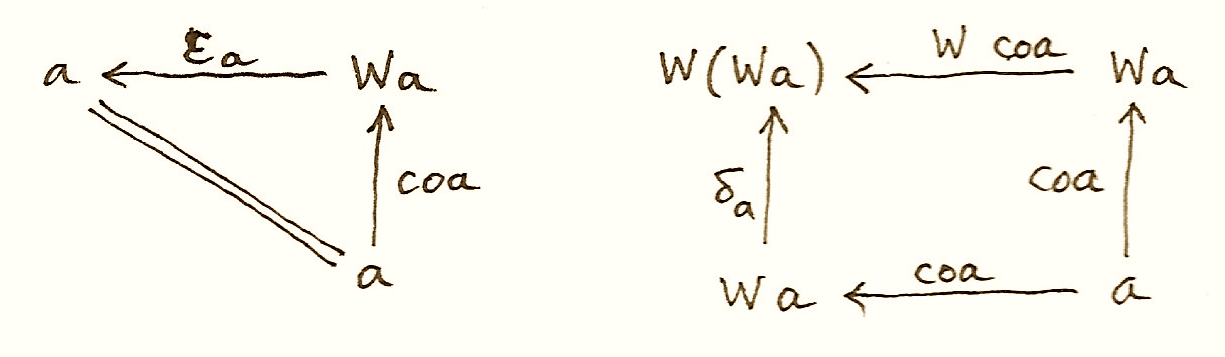
\includegraphics[width=4.67708in]{images/talg5.png}

where \code{coa} is the coevaluation morphism of the coalgebra whose
carrier is \code{a}:

\begin{verbatim}
coa :: a -> W a
\end{verbatim}

and \code{ε} and \code{δ} are the two natural transformations
defining the comonad (in Haskell, their components are called
\code{extract} and \code{duplicate}).

There is an obvious forgetful functor \code{UW} from the category of
these coalgebras to \emph{C}. It just forgets the coevaluation. We'll
consider its right adjoint \code{FW}.

\begin{verbatim}
UW ⊣ FW
\end{verbatim}

The right adjoint to a forgetful functor is called a cofree functor.
\code{FW} generates cofree coalgebras. It assigns, to an object
\code{a} in \emph{C}, the coalgebra \code{(W\ a,\ δa)}. The
adjunction reproduces the original comonad as the composite
\code{FW\ ∘\ UW}.

Similarly, we can construct a co-Kleisli category with co-Kleisli arrows
and regenerate the comonad from the corresponding adjunction.

\subsection{Lenses}\label{lenses}

Let's go back to our discussion of lenses. A lens can be written as a
coalgebra:

\begin{verbatim}
coalgs :: a -> Store s a
\end{verbatim}

for the functor \code{Store\ s}:

\begin{verbatim}
data Store s a = Store (s -> a) s
\end{verbatim}

This coalgebra can be also expressed as a pair of functions:

\begin{verbatim}
set :: a -> s -> a get :: a -> s
\end{verbatim}

(Think of \code{a} as standing for ``all,'' and \code{s} as a
``small'' part of it.) In terms of this pair, we have:

\begin{verbatim}
coalgs a = Store (set a) (get a)
\end{verbatim}

Here, \code{a} is a value of type \code{a}. Notice that partially
applied \code{set} is a function \code{s-\textgreater{}a}.

We also know that \code{Store\ s} is a comonad:

\begin{verbatim}
instance Comonad (Store s) where extract (Store f s) = f s duplicate (Store f s) = Store (Store f) s
\end{verbatim}

The question is: Under what conditions is a lens a coalgebra for this
comonad? The first coherence condition:

\begin{verbatim}
εa ∘ coalg = ida
\end{verbatim}

translates to:

\begin{verbatim}
set a (get a) = a
\end{verbatim}

This is the lens law that expresses the fact that if you set a field of
the structure \code{a} to its previous value, nothing changes.

The second condition:

\begin{verbatim}
fmap coalg ∘ coalg = δa ∘ coalg
\end{verbatim}

requires a little more work. First, recall the definition of
\code{fmap} for the \code{Store} functor:

\begin{verbatim}
fmap g (Store f s) = Store (g . f) s
\end{verbatim}

Applying \code{fmap\ coalg} to the result of \code{coalg} gives us:

\begin{verbatim}
Store (coalg . set a) (get a)
\end{verbatim}

On the other hand, applying \code{duplicate} to the result of
\code{coalg} produces:

\begin{verbatim}
Store (Store (set a)) (get a)
\end{verbatim}

For these two expressions to be equal, the two functions under
\code{Store} must be equal when acting on an arbitrary \code{s}:

\begin{verbatim}
coalg (set a s) = Store (set a) s
\end{verbatim}

Expanding \code{coalg}, we get:

\begin{verbatim}
Store (set (set a s)) (get (set a s)) = Store (set a) s
\end{verbatim}

This is equivalent to two remaining lens laws. The first one:

\begin{verbatim}
set (set a s) = set a
\end{verbatim}

tells us that setting the value of a field twice is the same as setting
it once. The second law:

\begin{verbatim}
get (set a s) = s
\end{verbatim}

tells us that getting a value of a field that was set to \code{s}
gives \code{s} back.

In other words, a well-behaved lens is indeed a comonad coalgebra for
the \code{Store} functor.

\subsection{Challenges}\label{challenges}

\begin{enumerate}
\item
  What is the action of the free functor
  \code{F\ ::\ C\ -\textgreater{}\ CT} on morphisms. Hint: use the
  naturality condition for monadic \code{μ}.
\item
  Define the adjunction:

\begin{verbatim}
UW ⊣ FW
\end{verbatim}
\item
  Prove that the above adjunction reproduces the original comonad.
\end{enumerate}

\subsection{Acknowledgment}\label{acknowledgment}

I'd like to thank Gershom Bazerman for helpful comments.

Next:
\href{https://bartoszmilewski.com/2017/03/29/ends-and-coends/}{Ends and
Coends}.
